\documentclass[../masters.tex]{subfiles}

\begin{document}
\graphicspath{{./imgs/}{../imgs/}} %look for images

\section{Nonlinear Models}
In this section we still consider probabilistic graphical models of the form shown in Figure \ref{fig_nlmod}. The variables retain their meaning as before but we generalise the model by dropping the linearity assumption. Unfortunately, this generalisation, although allowing us to expand our investigation to a much more expressive class of models, makes closed form solutions to the inference problem intractable in general.   
\begin{figure}[H] 
\centering
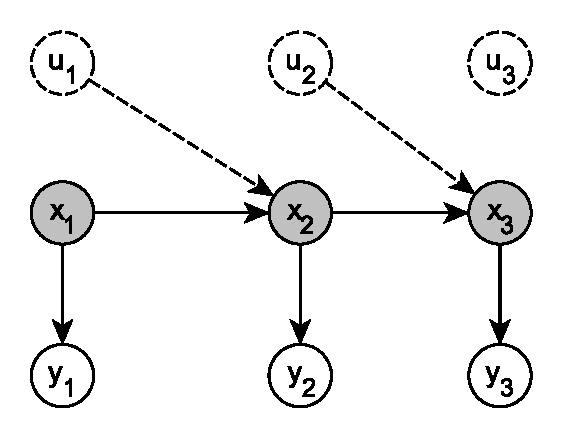
\includegraphics[scale=1.0]{linear_model.pdf}
\caption{Graphical model of this section}
\label{fig_nlmod}
\end{figure}
We again assume that the transition and emission functions are time invariant. The state space model is now of the form (\ref{eq_nlstatespace}).
\begin{equation}
\begin{aligned}
x_{t+1} &= f(x_t, u_t, w_{t+1}) \\
y_{t+1} &= g(x_{t+1}, v_{t+1})
\end{aligned}
\label{eq_nlstatespace}
\end{equation}
Note that we make no assumption about the functional form of the noise terms $w_t,v_t$. In practice it is customary to assume that they have zero mean but otherwise are not restricted. Additionally, to simplify notation we will omit the dependence on $u$ of $f$ and $g$ and their associated distributions. Since $u$ is a deterministic variable, by assumption, it is straightforward to incorporate it into later analysis. 

\subsection{Sequential Monte Carlo Methods}
Many approximate inference techniques exist in literature, the most notable ones include Gaussian Sum Filters \cite{gsf1} and Particle based methods. We shall focus only on Sequential Monte Carlo (SMC) methods, of which Particle based methods are a subset, because it is simple to implement and generalises well (and easily) to more complex graphical models. 

SMC methods are a general class of Monte Carlo methods which sample sequentially from the growing target distribution $\pi_t(x_{1:t})$. By only requiring that $\gamma_t$ be known point-wise we have the framework of SMC methods as shown in (\ref{eq_SMC1}). Note that $Z_t$ is some normalisation constant \cite{pftut}.
\begin{equation}
\begin{aligned}
\pi_t(x_{1:t}) &= \frac{\gamma_t(x_{1:t})}{Z_t} \\
Z_t &= \int_{x_{1:t}} \gamma_t(x_{1:t})
\end{aligned}
\label{eq_SMC1}
\end{equation} 
For example, in the context of filtering we have that $\gamma_t(x_{1:t}) = p(x_{1:t},y_{1:t})$ and $Z_t = p(y_{1:t})$ so that $\pi_t(x_{1:t}) = p(x_{1:t}|y_{1:t})$. 

It is possible to approximate the distribution $\pi_t(x_{1:t})$ by drawing $N$ samples $X_{1:t}^i \backsim \pi_t(x_{1:t})$ and using the Monte Carlo method to find the approximation $\hat{\pi}_t(x_{1:t})$ as shown in (\ref{eq_SMC2}).
\begin{equation}
\hat{\pi}_t(x_{1:t}) = \frac{1}{N}\sum_{i=1}^N \delta(X^i_{1:t}, x_{1:t})
\label{eq_SMC2}
\end{equation}
We denote the Dirac Delta function of $x$ with mass located at $x_0$ by $\delta(x_0,x)$. It is easy to approximate the marginal $\pi_t(x_{t})$ as shown in (\ref{eq_SMC3}).
\begin{equation}
\hat{\pi}_t(x_{t}) = \frac{1}{N}\sum_{i=1}^N \delta(X^i_{t}, x_{t})
\label{eq_SMC3}
\end{equation}
It can be shown that the variance of the approximation error of $\pi_t$ decreases at rate $\mathcal{O}(\frac{1}{N})$. Unfortunately there are two significant drawbacks to the Monte Carlo approximation. The first is that often we cannot sample from $\pi_t(x_{1:t})$ directly and the second is that even if we could it is often computationally prohibitive. 

We use the Importance Sampling method to address the first problem. We do this by introducing an importance (sometimes called proposal) density $q_t(x_{1:t})$ such that $\pi_t(x_{1:t}) > 0 \implies q_t(x_{1:t}) > 0$. By substituting this into the SMC framework (\ref{eq_SMC1}) we have (\ref{eq_SMC4}).
\begin{equation}
\begin{aligned}
\pi_t(x_{1:t}) &= \frac{w_t(x_{1:t})q_t(x_{1:t})}{Z_t} \\
Z_t &= \int_{x_{1:t}} w_t(x_{1:t})q_t(x_{1:t})
\end{aligned}
\label{eq_SMC4}
\end{equation} 
Where we have defined the unnormalised weight function $w_t(x_{1:t}) = \frac{\gamma_t(x_{1:t})}{q_t(x_{1:t})}$. It is possible, for example, to set $q_t$ to a multivariate Gaussian which is easy to sample from. By drawing $N$ samples $X_{1:t}^i \backsim q_t(x_{1:t})$ and using (\ref{eq_SMC4}) we have (\ref{eq_SMC5}). 
\begin{equation}
\begin{aligned}
\hat{\pi}_t(x_{1:t}) &= \frac{1}{N}\sum_{i=1}^N W_t^i\delta(X^i_{1:t}, x_{1:t}) \\
\hat{Z}_t &= \frac{1}{N}\sum_{i=1}^N w_t(X^i_{1:t}) \\
W^i_t &= \frac{w_t(X^i_{1:t})}{\sum_{i=1}^N w_t(X^i_{1:t})}
\end{aligned}
\label{eq_SMC5}
\end{equation}
Now we will attempt to modify the Importance Sampling method to address the second problem of computational cost incurred by the sampling routine. 

We do this by selecting an importance/proposal distribution which factorises according to $q_t(x_{1:t}) = q_{t-1}(x_{1:t-1})q_t(x_{t}|x_{1:t-1}) = q_1(x_1) \Pi_{k=2}^t q_k(x_k|x_{1:k-1})$. In this way we only need to sample sequentially at each time step: at time $t=1$ we sample $X_1^i \backsim q_1(x_1)$, at time $t=2$ we sample $X_{2}^i \backsim q_2(x_2|x_1)$ and so we build up $X^i_{1:t} \backsim q_t(x_{1:t})$ factor by factor.

The weights can be written in the form (\ref{eq_SMC6}).
\begin{equation}
\begin{aligned}
w_t(x_{1:t}) &= \frac{\gamma_t(x_{1:t})}{q_t(x_{1:t})} \\
&= \frac{\gamma_{t-1}(x_{1:t-1})}{q_{t-1}(x_{1:t-1})}\frac{\gamma_t(x_{1:t})}{\gamma_{t-1}(x_{1:t-1})q_t(x_t|x_{1:t-1})} \\
&= w_{t-1}(x_{1:t-1})\alpha_t(x_{1:t-1}) \\
&= w_1(x_1)\Pi_{k=2}^t \alpha_k(x_{1:k})
\end{aligned}
\label{eq_SMC6}
\end{equation}
Thus, at any time $t$ we can obtain the estimates $\hat{\pi}_t(x_{1:t})$ and $Z_t$. The major limitation of this approach is that the variance of the resulting estimates typically increases exponentially with $t$ \cite{pftut}. 

We overcome this problem by resampling and thus introduce the Sequential Importance Resampling (SIR) method. So far we have a set of weighted samples generated from $q_t(x_{1:t})$ which builds the approximation $\hat{\pi}_t(x_{1:t})$. However, sampling directly from $\hat{\pi}_t(x_{1:t})$ does not approximate $\pi_t(x_{1:t})$. To obtain an approximate distribution of $\pi_t(x_{1:t})$ we need to sample from the weighted distribution $\hat{\pi}_t(x_{1:t})$. This is called resampling because we are sampling from a sampled distribution. Many techniques exist to perform this step efficiently. The crudest and most widely used one is to simply use the discrete multinomial distribution based on $W^i_{1:t}$ to draw samples from $\hat{\pi}_t(x_{1:t})$ \cite{pftut}. 

The benefit of resampling is that it allows us to remove particles with low weight and thus keeps the variance of the estimate in check. We are finally ready to consider the general SIR  algorithm:

\textbf{SIR Algorithm} \\
For $t=1$:
\begin{enumerate}
\item
Sample $X^i_1 \backsim q_1(x_1)$.
\item
Compute the weights $w_1(X_1^i)$ and $W^i_1 \propto w_1(X^i_1)$.
\item
Resample $(W^i_1, X^i_1)$ to obtain $N$ equally weighted particles $(\frac{1}{N}, \bar{X}^i_1)$.
\end{enumerate}
For $t \geq 2$:
\begin{enumerate}
\item
Sample $X^i_t \backsim q_t(x_t|\bar{X}^i_{1:t-1})$ and set ${X}^i_{1:t} \leftarrow (\bar{X}^i_{1:t-1}, X^i_t)$ .
\item
Compute the weights $\alpha_t(X^i_{1:t})$ and $W^i_t \propto \alpha_t(X^i_{1:t})$.
\item
Resample $(W^i_t, X^i_{1:t})$ to obtain $N$ equally weighted particles $(\frac{1}{N}, \bar{X}^i_{1:t})$.
\end{enumerate}
At any time $t$ we have two approximations for $\pi(x_{1:t})$ as shown in (\ref{eq_smc_algo}).
\begin{equation}
\begin{aligned}
\hat{\pi}(x_{1:t}) &= \sum_{i=1}^N W^i_t \delta(X^i_{1:t}, x_{1:t}) \\
\bar{\pi}(x_{1:t}) &= \frac{1}{N}\sum_{i=1}^N \delta(\bar{X}^i_{1:t}, x_{1:t})
\end{aligned}
\label{eq_smc_algo}
\end{equation}
The latter approximation represents the resampled estimate and the former represents the sampled estimate \cite{pftut}. We prefer the former because in the limit as $N \rightarrow \infty$ it is a better approximation of $\pi_t$. However, as we have mentioned the variance of $\hat{\pi}(x_{1:t})$ tends to be unbounded and thus we often have that most of the particles in the particle population have very low weight. From a computational point of view this is wasteful. To ameliorate this we use the latter, resampled, estimate. However, the problem with the resampled estimate is that it effectively culls low weight particles and this reduces the diversity of the particle population \cite{murphy1}. 

We attempt to get the benefit of both worlds by only performing resampling when the weight variance of the particles becomes large. The Effective Sample Size (ESS) is a method whereby one determines when to perform resampling according to (\ref{eq_ess}).
\begin{equation}
\text{ESS} = \frac{1}{\sum_{i=1}^N (W^i_n)^2}
\label{eq_ess}
\end{equation} 
If the ESS becomes smaller than some threshold (typically $\frac{N}{2}$) we resample to cull low weight particles and replace them with high weight particles. In this manner we have a computationally feasible method. This is called adaptive resampling and is a straightforward extension of the SMC algorithm as shown below.

\textbf{Adaptive SIR Algorithm}\\
For $t=1$:
\begin{enumerate}
\item
Sample $X^i_1 \backsim q_1(x_1)$.
\item
Compute the weights $w_1(X_1^i)$ and $W^i_1 \propto w_1(X^i_1)$.
\item
If resample criterion is satisfied then resample $(W^i_1, X^i_1)$ to obtain $N$ equally weighted particles $(\frac{1}{N}, \bar{X}^i_1)$ and set $(\bar{W}^i_1, \bar{X}^i_1) \leftarrow (\frac{1}{N}, \bar{X}^i_1)$ otherwise set $(\bar{W}^i_1, \bar{X}^i_1) \leftarrow ({W}^i_1, {X}^i_1)$.
\end{enumerate}
For $t \geq 2$:
\begin{enumerate}
\item
Sample $X^i_t \backsim q_t(x_t|\bar{X}^i_{1:t-1})$ and set ${X}^i_{1:t} \leftarrow (\bar{X}^i_{1:t-1}, X^i_t)$ .
\item
Compute the weights $\alpha_t(X^i_{1:t})$ and $W^i_t \propto \bar{W}^i_{t-1}\alpha_t(X^i_{1:t})$.
\item
If the resample criterion is satisfied then resample $(W^i_t, X^i_{1:t})$ to obtain $N$ equally weighted particles $(\frac{1}{N}, \bar{X}^i_{1:t})$ and set $(\bar{W}^i_1, \bar{X}^i_t) \leftarrow (\frac{1}{N}, \bar{X}^i_t)$ otherwise set $(\bar{W}^i_t, \bar{X}^i_t) \leftarrow ({W}^i_t, {X}^i_t)$.
\end{enumerate}

Numerous convergence results exist for the SMC methods we have discussed but the fundamental problem with this scheme is that of sample impoverishment. It is fundamentally impossibly to accurately represent a distribution on a space of arbitrarily high dimension with a finite set of samples \cite{pftut}. We attempt to mitigate this problem by using resampling but degeneracy inevitably occurs for large enough $t$. Fortunately, for our purposes we will not be dealing with arbitrarily large dimensional problems because of the Markov assumption.

\subsection{Particle Filter}
We now apply the adaptive SIR algorithm in the setting of filtering. We set $\pi_t(x_{1:t}) = p(x_{1:t}|y_{1:t})$, $\gamma_t(x_{1:t}) = p(x_{1:t}, y_{1:t})$ and consequently $Z_t = p(y_{1:t})$. We use the recursive proposal distribution $q_t(x_{1:t}|y_{1:t}) = q(x_t|x_{1:t-1}, y_{1:t})q_{t-1}(x_{1:t-1}|y_{1:t-1})$. We then have the unnormalised weights as shown in (\ref{eq_pf_weights}).
\begin{equation}
\begin{aligned}
w_t(x_{1:t}) &= \frac{\gamma_t(x_{1:t})}{q_t(x_{1:t}|y_{1:t})} \\
&= \frac{p(x_{1:t}, y_{1:t})}{q_t(x_{1:t}|y_{1:t})} \\
&\propto \frac{p(x_{1:t}| y_{1:t})}{q_t(x_{1:t}|y_{1:t})} \\
&\propto \frac{p(y_t|x_t)p(x_t|x_{t-1})}{q_t(x_t|x_{1:t-1}, y_{1:t})}\frac{p(x_{1:t-1}| y_{1:t-1})}{q_{t-1}(x_{1:t-1}|y_{1:t-1})} \\
&= \alpha_t(x_{1:t})w_{t-1}(x_{1:t-1})
\end{aligned}
\label{eq_pf_weights}
\end{equation}
For filtering we only care about $p(x_t|y_{1:t})$ and thus we do not need the entire trajectory $x_{1:t}$. The proposal distribution then simplifies $q_t(x_t|x_{1:t-1}, y_{1:t}) = q_t(x_{t}|x_{t-1}y_{t})$. In this case the incremental weight $\alpha_t$ simplifies to (\ref{eq_pf_simpweights}).
\begin{equation}
\alpha_t(x_t) = \frac{p(y_t|x_t)p(x_t|x_{t-1})}{q_t(x_t|x_{t-1}, y_{t})} 
\label{eq_pf_simpweights}
\end{equation}
The most common proposal distribution is, the suboptimal, $q_t(x_t|x_{t-1}|y_t) = p(x_t|x_{t-1})$ because it is easy to sample from. This implies that the incremental weights simplify to $\alpha_t(x_t) = p(y_t|x_t)$. Using such a proposal distribution was initially proposed in \cite{gordon} in the setting of the non-adaptive SIR method. 

For general purpose filtering this is not very efficient because it amounts to ``guessing until you hit". If the transitions are very stochastic inference can be improved by using the optimal proposal distribution $q_t(x_t|x_{t-1}, y_t) = p(x_t|x_{t-1}, y_t)$. While this is optimal it introduces some difficulty because, in general, it is more difficult to sample from. The focus of dissertation is not on optimal filtering and for the purposes of prediction the suggested proposal distribution is sufficiently good \cite{murphy1}. We thus restrict ourselves to the proposal distribution $p(x_t|x_{t-1})$ for simplicity.

Finally, we have mentioned that resampling kills off unlikely particles. An unfortunate consequence of this is that some particle diversity is lost. An empirical method used to attenuate this problem is to resample from a kernel around the particle selected by the resampling process. This is called roughening in \cite{gordon}. We thus make a final modification to the adaptive SIR algorithm. We select a particle from the population in the standard way but resample from a Normal distribution centred around that particle and with a diagonal covariance matrix where the standard deviation of each diagonal is $KEN^{-\frac{1}{d}}$. We define $E$ as the range of the particle's relevant component, $N$ as the number of particles and $d$ as the dimension of the problem. $K$ is a tuning factor which specifies how broad the kernel we sample from should be. 

For the sake of completeness we present the Particle Filter algorithm we used here. Recall that $f$ and $g$ are the transition and observation functions respectively. The algorithm is applied to each particle $i=1,2,...,N$.

\textbf{Particle Filter Algorithm}\\
For $t=1$:
\begin{enumerate}
\item
Sample $X^i_1 \backsim p(x_1)$.
\item
Compute the weights $w_1(X_1^i) = p(Y^*_1|X_1^i) = \mathcal{N}(Y^*_1|g(X^i_1), \text{covar}[v_1])$ where $Y^*_1$ is the observation. Normalise $W^i_1 \propto w_1(X^i_1)$.
\item
If the number of effective particles is below some threshold apply resampling with roughening $(W^i_1, X^i_1)$ to obtain $N$ equally weighted particles $(\frac{1}{N}, \bar{X}^i_1)$ and set $(\bar{W}^i_1, \bar{X}^i_1) \leftarrow (\frac{1}{N}, \bar{X}^i_1)$ otherwise set $(\bar{W}^i_1, \bar{X}^i_1) \leftarrow ({W}^i_1, {X}^i_1)$
\end{enumerate}
For $t \geq 2$:
\begin{enumerate}
\item
Sample $X^i_t = f(\bar{X}^i_{t-1}, w_t) \backsim p(x_t|\bar{X}^i_{t-1})$.
\item
Compute the weights $\alpha_t(X^i_{t}) = p(Y^*_t|X_t^i) = \mathcal{N}(Y^*_t|g(X^i_t), \text{covar}[v_t])$ and normalise $W^i_t \propto \bar{W}^i_{t-1}\alpha_t(X^i_{t})$.
\item
If the number of effective particles is below some threshold apply resampling with roughening $(W^i_t, X^i_{t})$ to obtain $N$ equally weighted particles $(\frac{1}{N}, \bar{X}^i_{t})$ and set $(\bar{W}^i_1, \bar{X}^i_t) \leftarrow (\frac{1}{N}, \bar{X}^i_t)$ otherwise set $(\bar{W}^i_t, \bar{X}^i_t) \leftarrow ({W}^i_t, {X}^i_t)$.
\end{enumerate}
The algorithm presented above is a slight generalisation of the bootstrap Particle Filter as initially proposed by Gordon et. al. \cite{gordon}.

Intuitively the algorithm may be summarised like this. Particle Filters predict the next hidden state by projecting all the current particles forward using the transition function. For each particle the likelihood of the observation is calculated given the particle and measurement noise. This likelihood is related to the weight of each particle. Particles with a relatively high weight are then deemed to more accurately represent the posterior distribution and thus we infer the posterior state estimate based on the relative weights of each particle.

\subsection{Particle Prediction}
We are primarily interested in predicting the future hidden states but we also show how the future visible states may be predicted within the framework of Particle methods. Recalling the prediction derivations of the Hidden Markov Model section and the Linear Models section we expect the hidden state prediction to merely be an $n$ step ahead projection of the current filtered particles. Likewise, we expect the visible state prediction to just be transformation of the predicted hidden states under the emission function. 

Inspecting the bootstrap Particle Filter algorithm presented in the previous subsection we are relieved to find that this is the case. One just removes the observation update steps (steps 2 and 3) from the algorithm because we cannot observe the future. We illustrate the two step ahead predictions and trust that the reader understand what we mean.

\textbf{Particle Prediction Algorithm}
\begin{enumerate}
\item
Sample $X_{t+1}^i = f(\bar{X}_t^i, w_{t+1}) \backsim p(x_{t+1}^i|y_t, \bar{X}_t^i)$ 
\item
Project $X_{t+2}^i = f(X_{t+1}^i, w_{t+2}) \backsim p(x_{t+2}^i|y_t, X_{t:t+1}^i)$ 
\item
Project $Y_{t+2}^i = g(X_{t+2}^i, v_{t+2}) \backsim p(y_{t+2}^i|y_t, X_{t:t+1}^i)$ 
\end{enumerate}

\subsection{Smoothing and Viterbi Decoding}
In the context of nonlinear transition and emission functions smoothing and Viterbi decoding are much more difficult than before. For the purposes of this dissertation it is not important to consider inferences of that type and thus we merely refer the reader to literature where this is discussed \cite{pftut}\cite{gsf1}\cite{murphy1}\cite{murphy2}\cite{barber}.

\subsection{Filtering the CSTR}
In this section we apply the Particle Filter to the nonlinear CSTR problem. We first demonstrate the effectiveness of the Particle Filter by performing inference using the full nonlinear CSTR model (measuring both the temperature and concentration). Next we use the full nonlinear model again but only measure temperature. Finally, we apply the Particle Filter to the CSTR using the linear model and compare it to the Kalman Filter.

In Figure \ref{fig_pf_m2_time} we see the Particle Filter state estimates given  $\text{cov}[w_t] = \begin{pmatrix}
5\times 10^{-4} & 0 \\ 0 & 10
\end{pmatrix}$ and $\text{cov}[v_t] = \begin{pmatrix}
5\times 10^{-3} & 0 \\ 0 & 15
\end{pmatrix}$. The noise covariances are appreciably more than what we used in the linear case to illustrate the robustness of the filter. We have used 500 particles to represent the estimated state posterior.
\begin{figure}[H] 
\centering
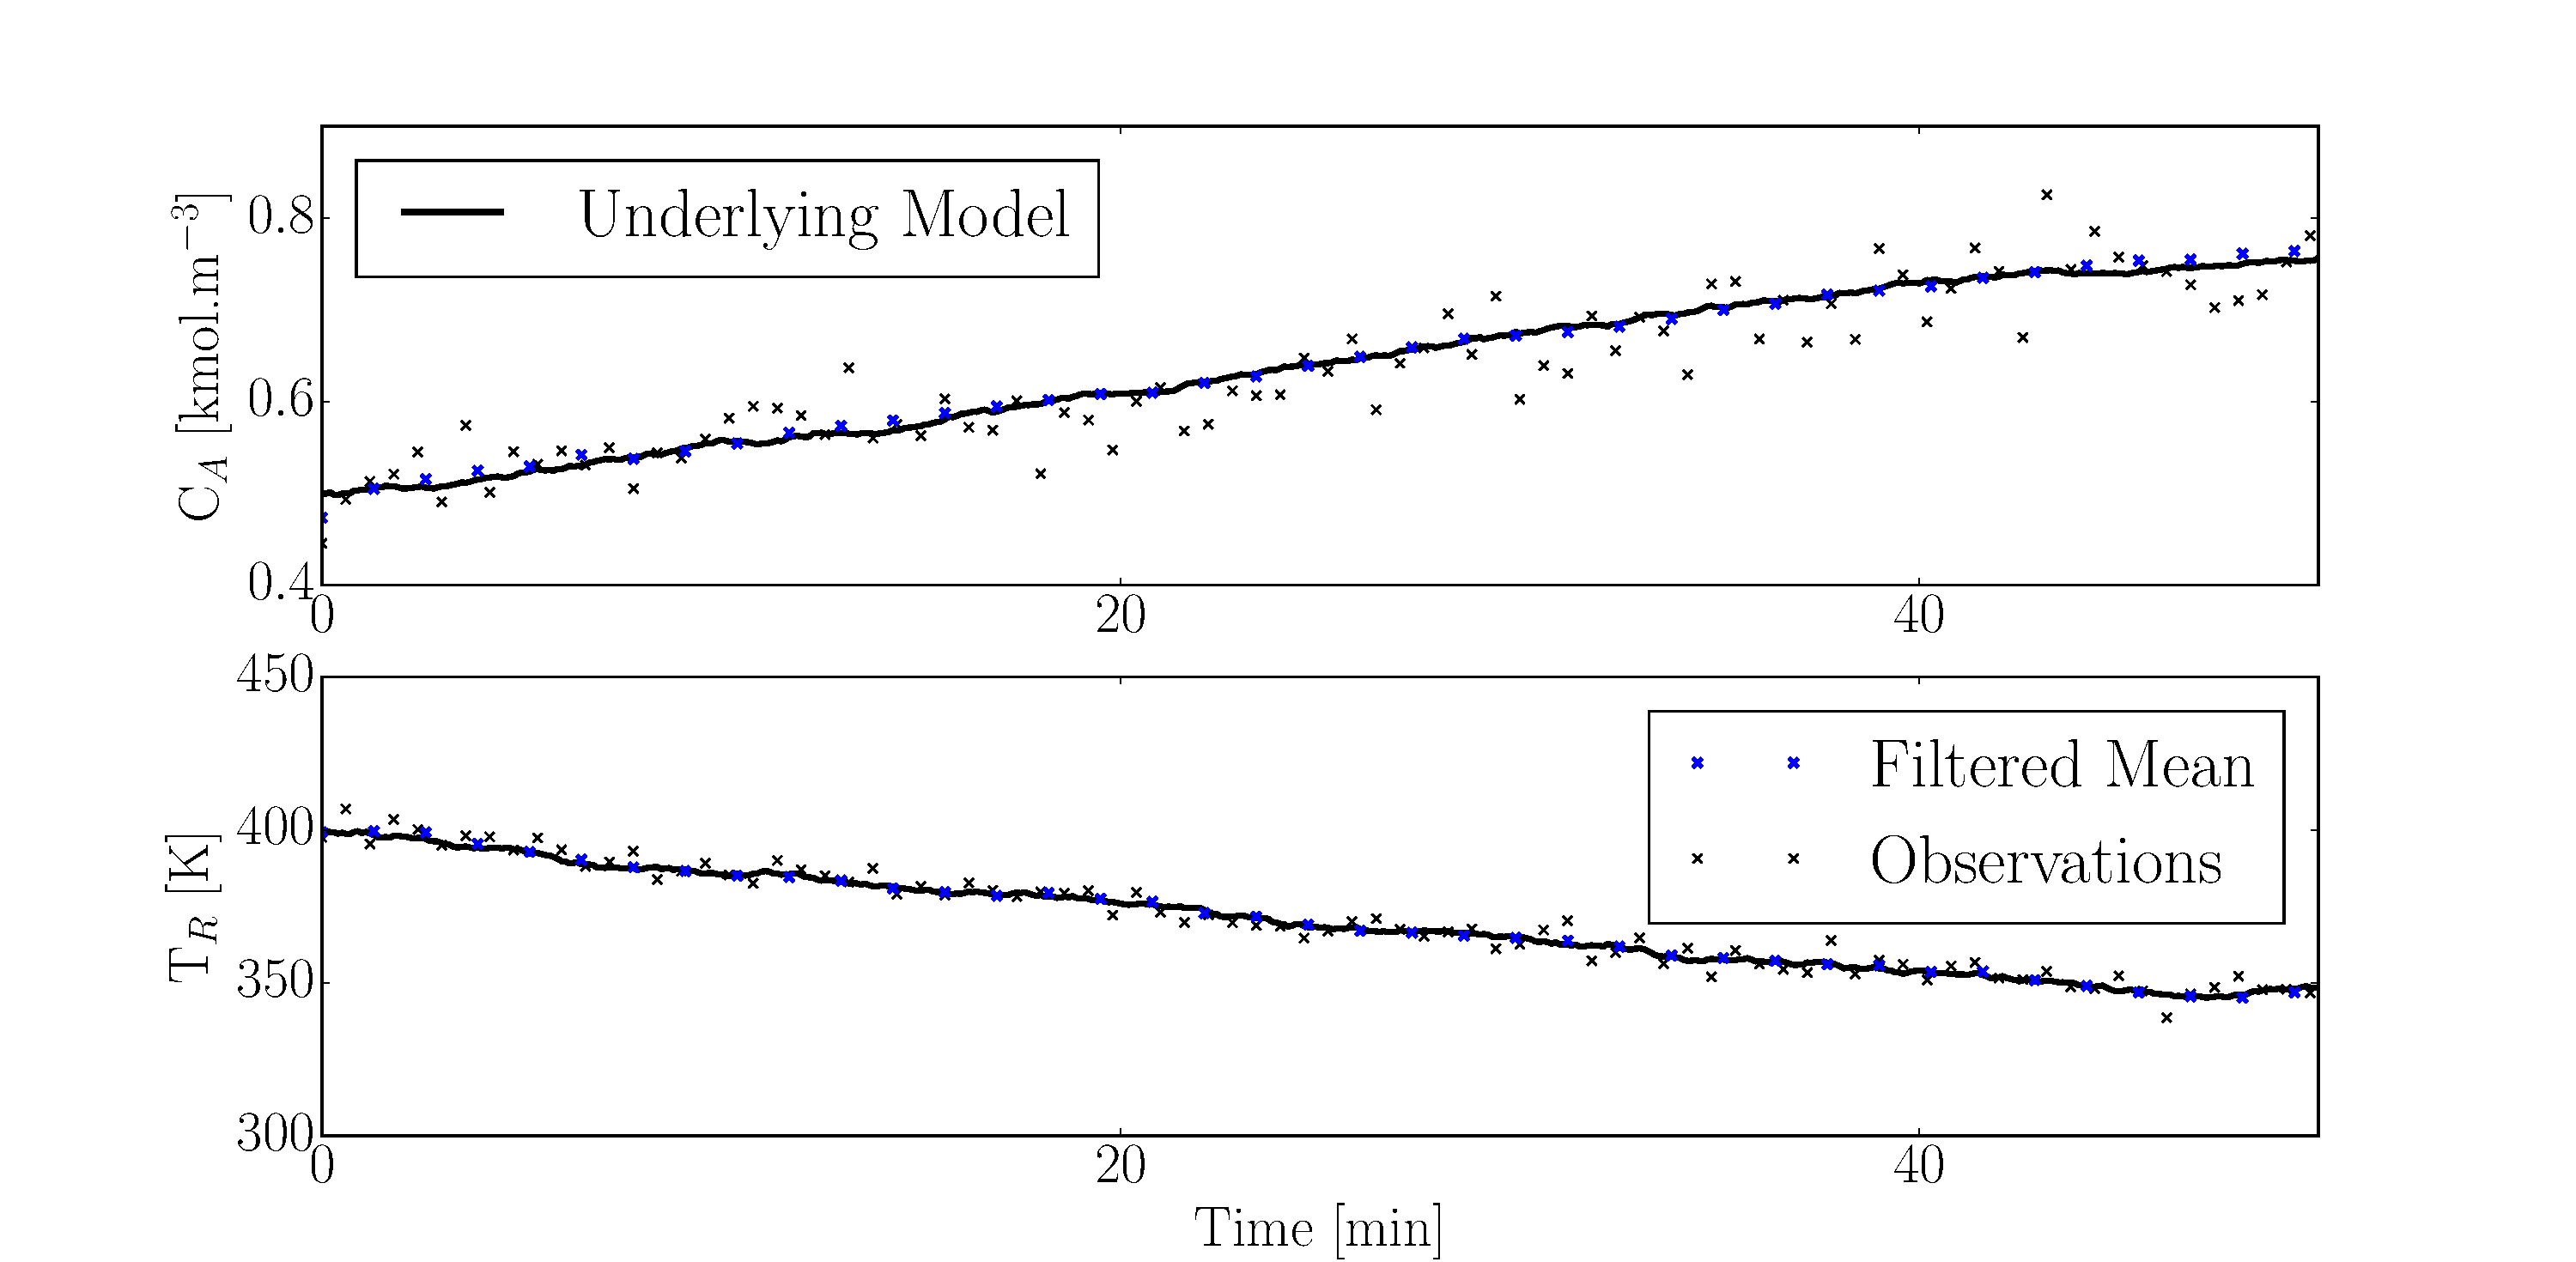
\includegraphics[scale=0.30]{pf_m2_time.pdf}
\caption{Time series state estimates using the Particle Filter on the nonlinear CSTR model with initial condition $(0.5, 450)$ and measuring both states.}
\label{fig_pf_m2_time}
\end{figure}
It is clear that that the filter reliably tracks the state evolution even in the presence of significant plant and measurement noise. For completeness we also show the state space evolution of the state estimate in Figure \ref{fig_pf_m2_phase}. 
\begin{figure}[H] 
\centering
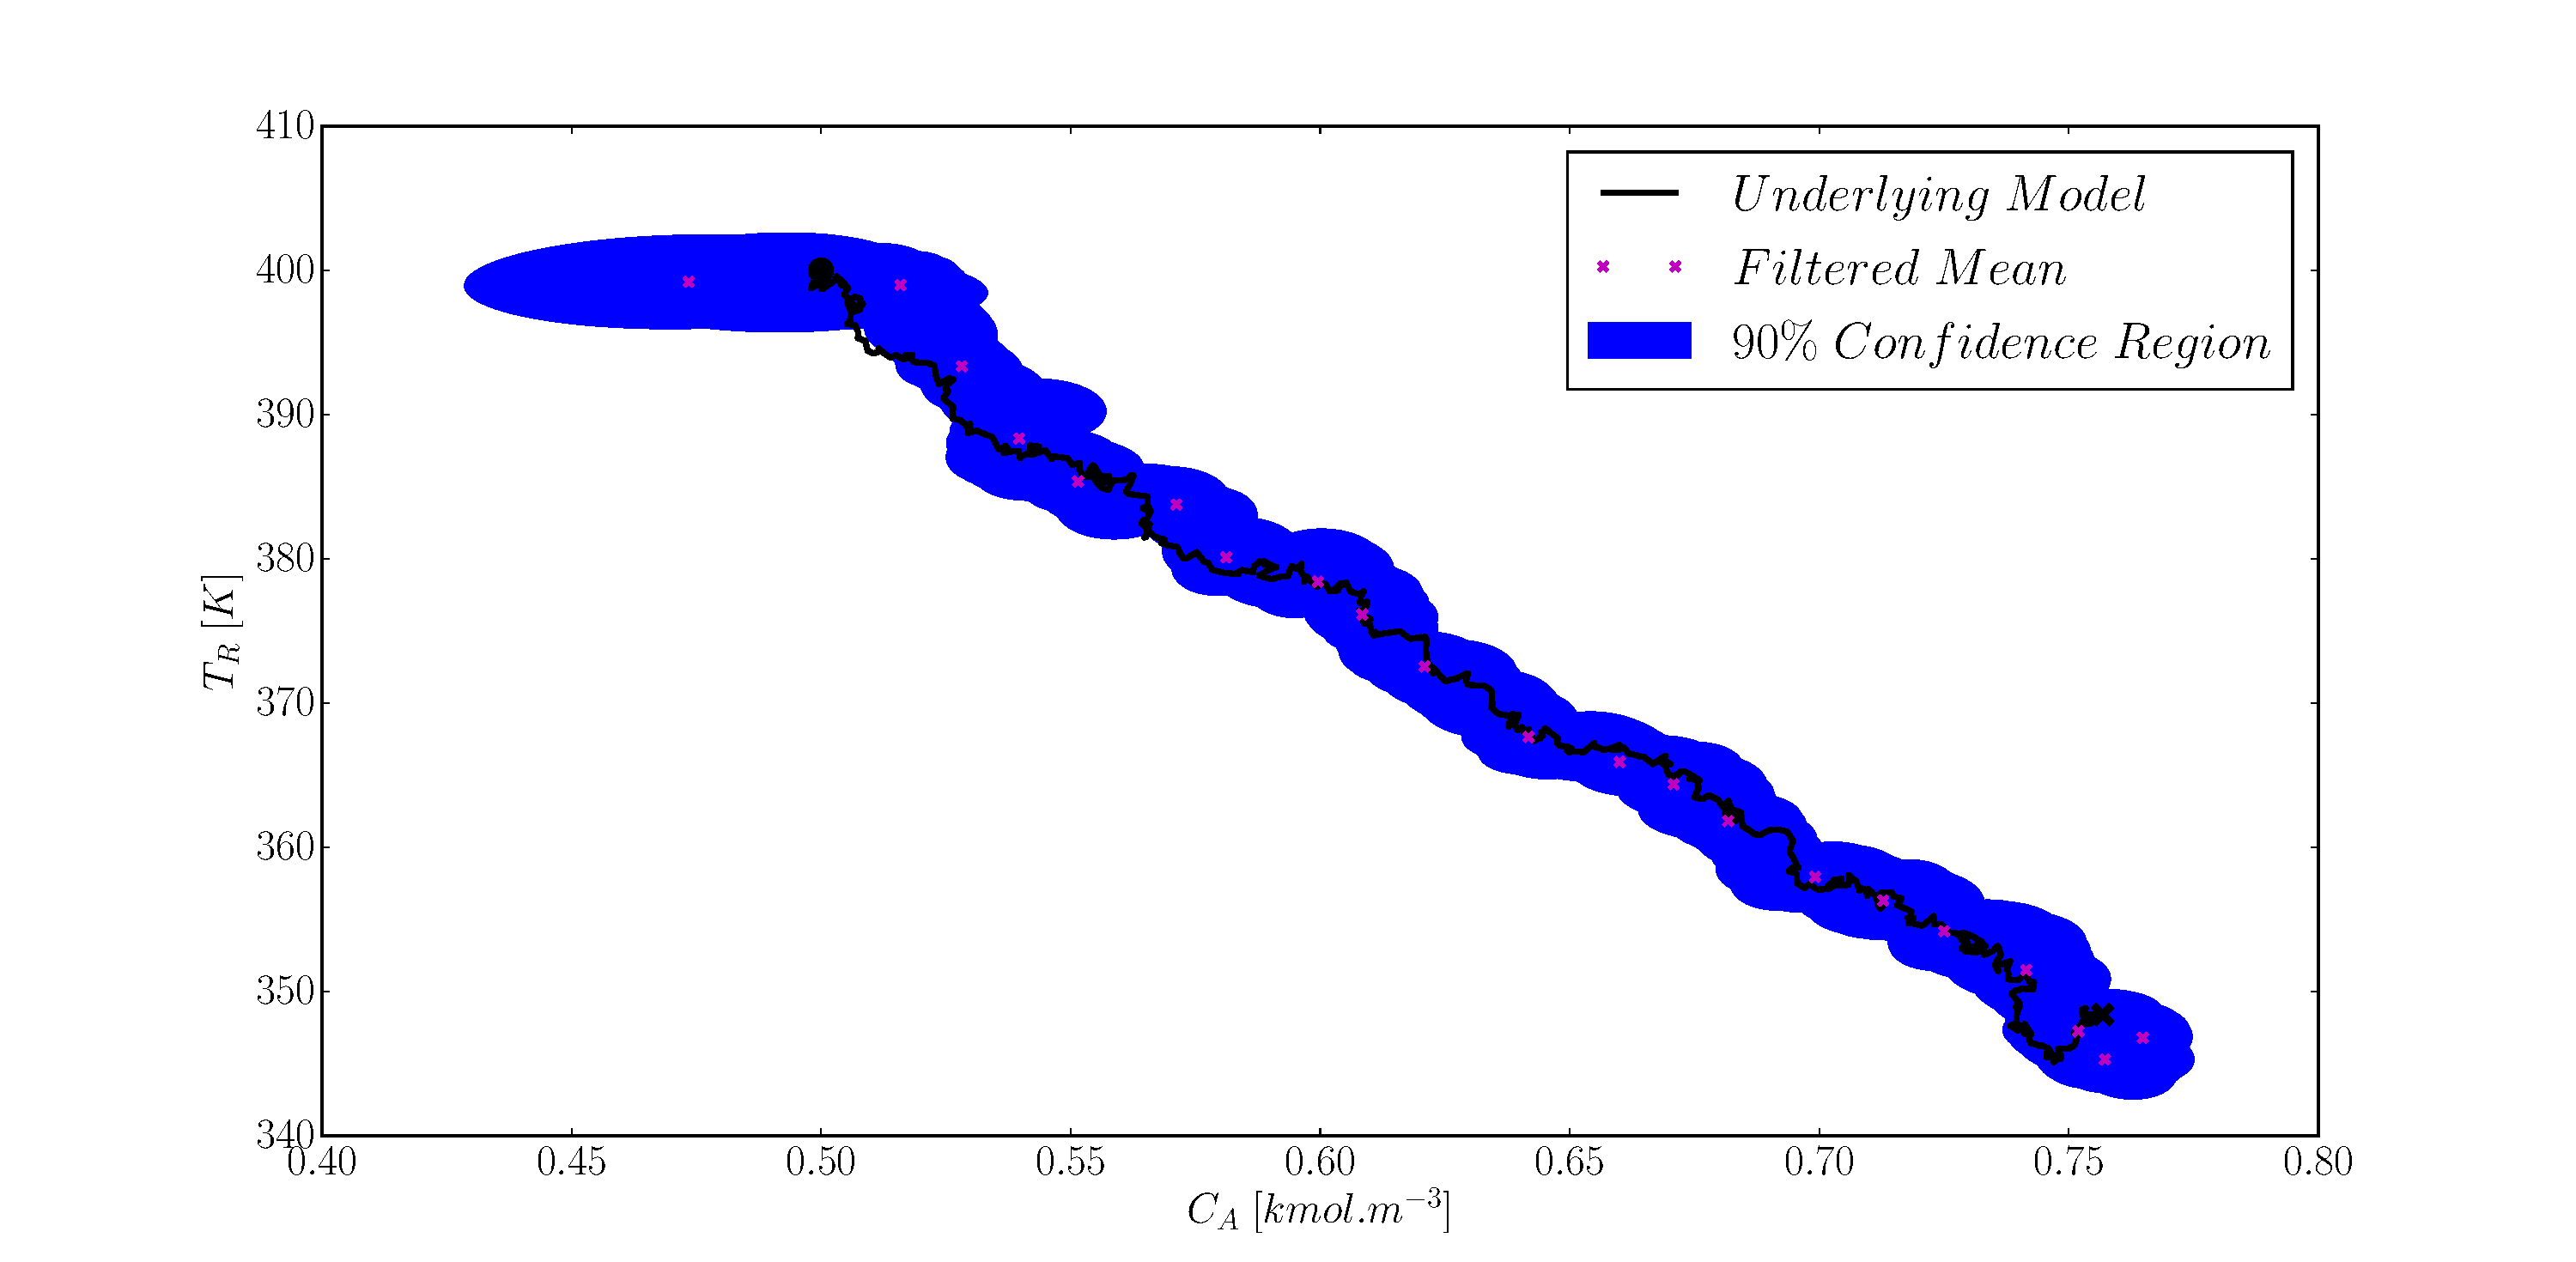
\includegraphics[scale=0.30]{pf_m2_phase.pdf}
\caption{State space evolution of the Particle Filter on the nonlinear CSTR model with initial condition $(0.5, 450)$ and measuring both states.}
\label{fig_pf_m2_phase}
\end{figure}
It is clear that the Particle Filter, using both measurements, is a robust and reliable state estimator. We now investigate if the Particle Filter, using the nonlinear model, performs well if only one measurement is made. We adjust the noise terms to $\text{cov}[w_t] = \begin{pmatrix}
1\times 10^{-4} & 0 \\ 0 & 4
\end{pmatrix}$ and $\text{cov}[v_t] = \begin{pmatrix} 10
\end{pmatrix}$ because we expect this inference task to be harder. In Figure \ref{fig_pf_m1_time} we see the state estimates as a function of time. Note that we have used 100 particles to represent the estimated state posterior.
\begin{figure}[H] 
\centering
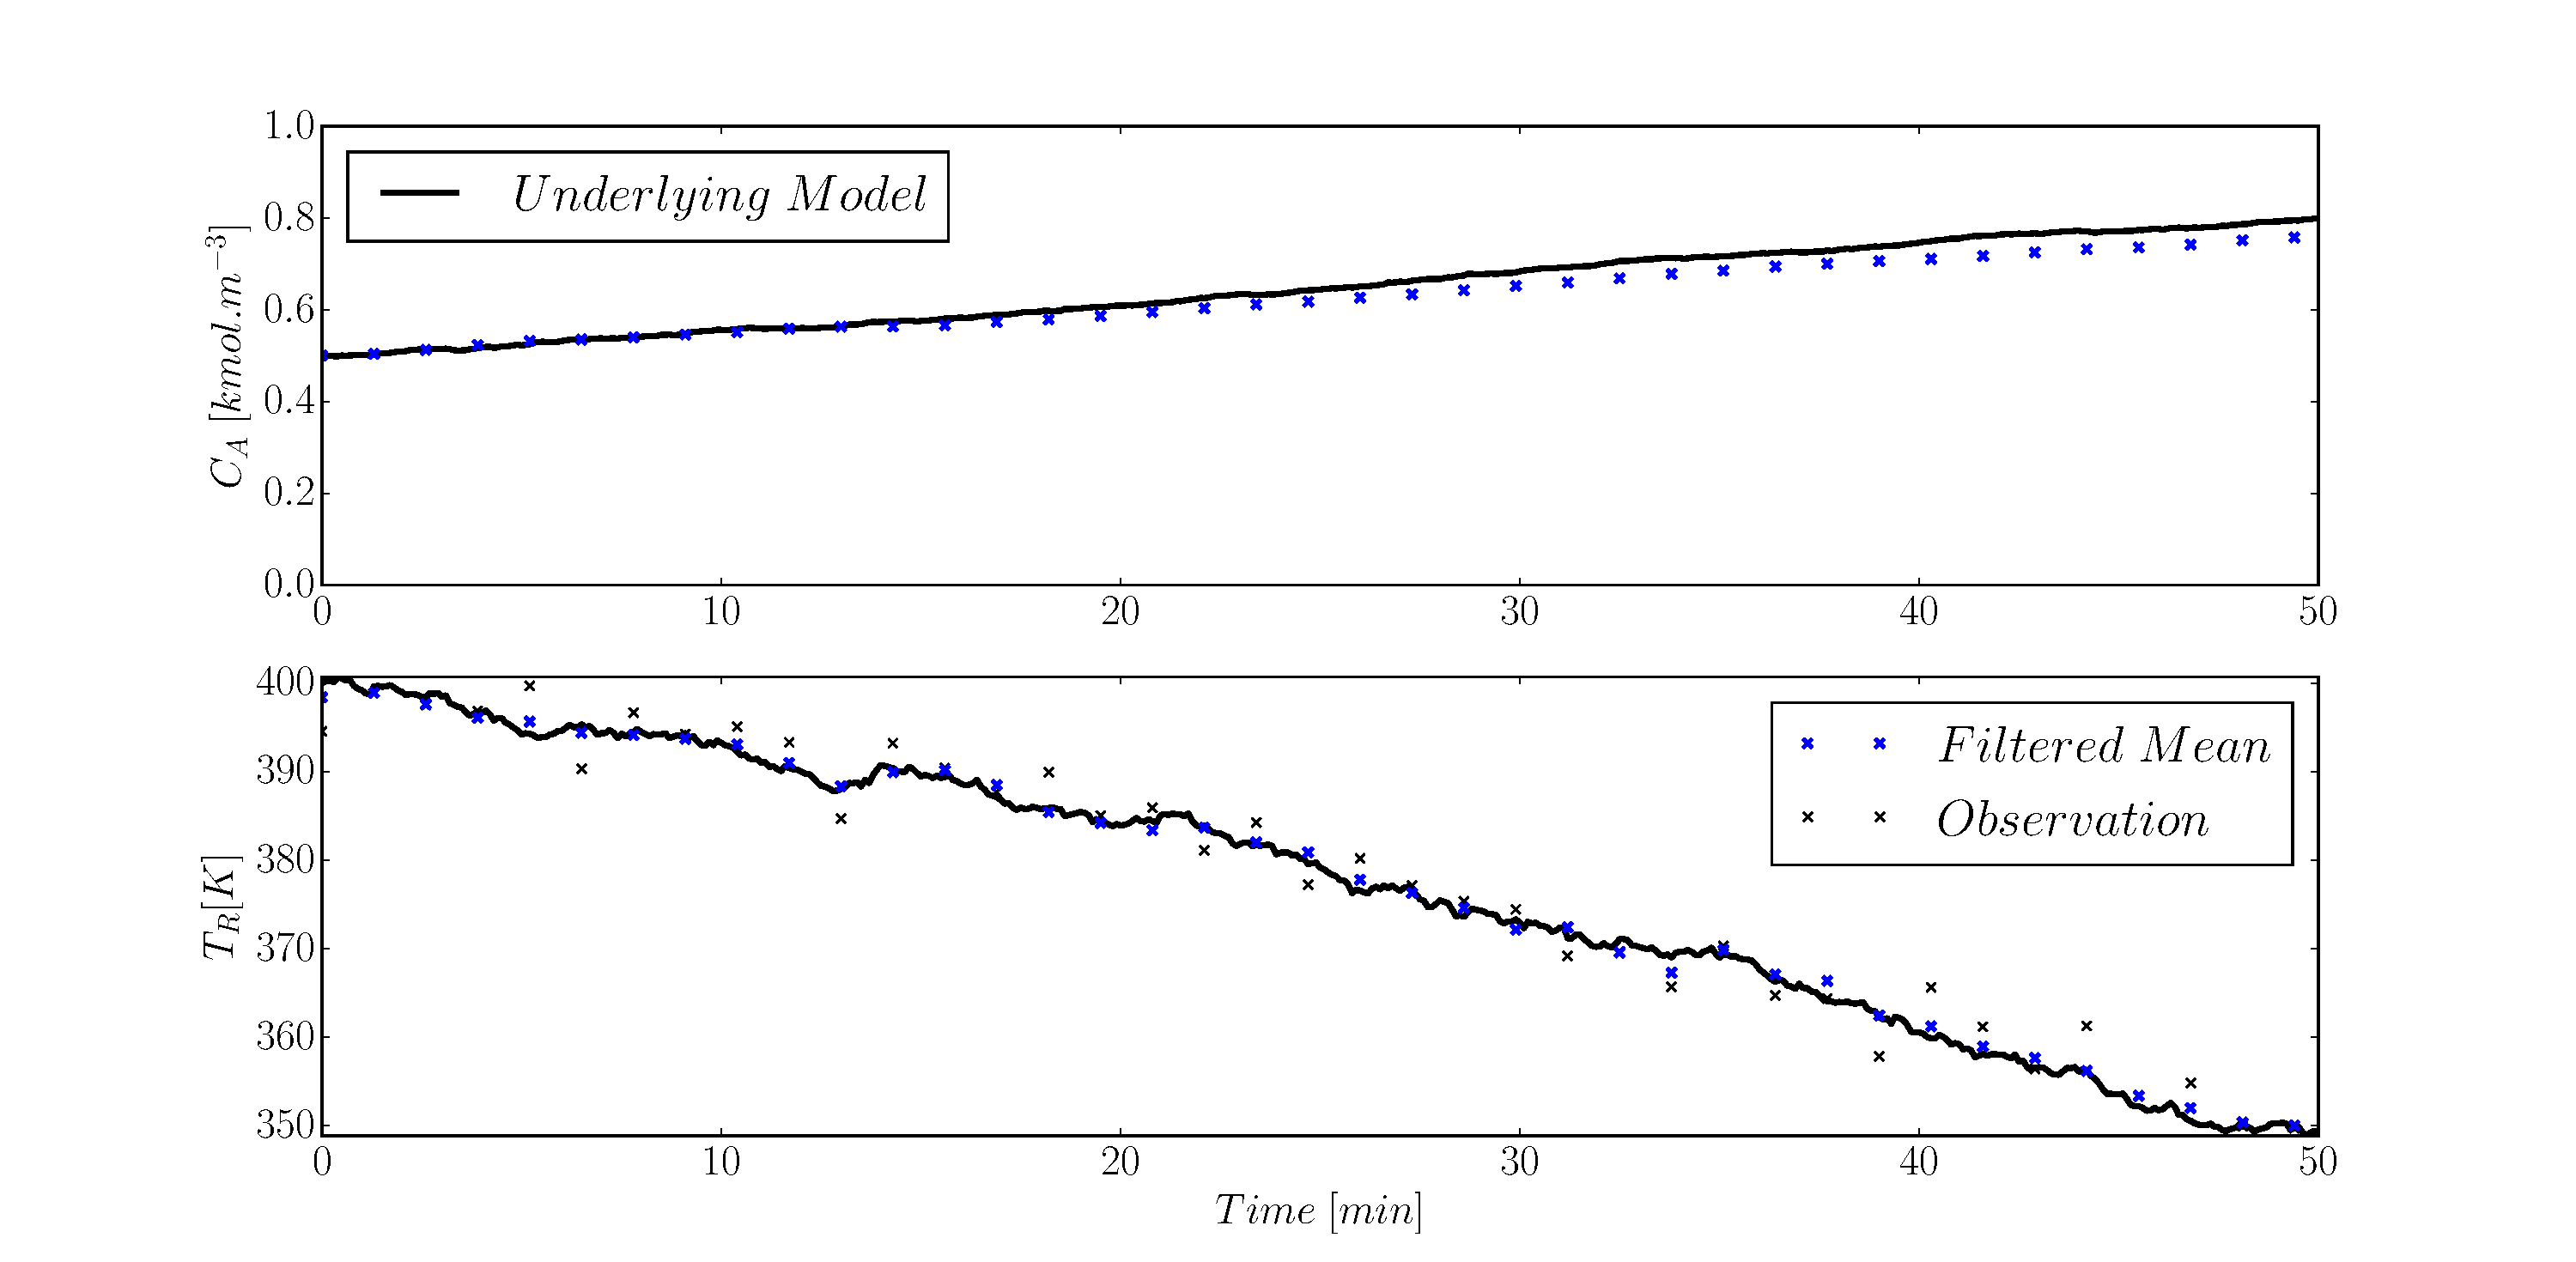
\includegraphics[scale=0.30]{pf_m1_time.pdf}
\caption{Time series state estimates using the Particle Filter on the nonlinear CSTR model with initial condition $(0.5, 450)$ and measuring only temperature.}
\label{fig_pf_m1_time}
\end{figure}
It seems as if the Filter struggles initially but soon weeds out and replaces the particles which do not support the state observations. This is reflected in the state space evolution curve in Figure \ref{fig_pf_m1_phase}.
\begin{figure}[H] 
\centering
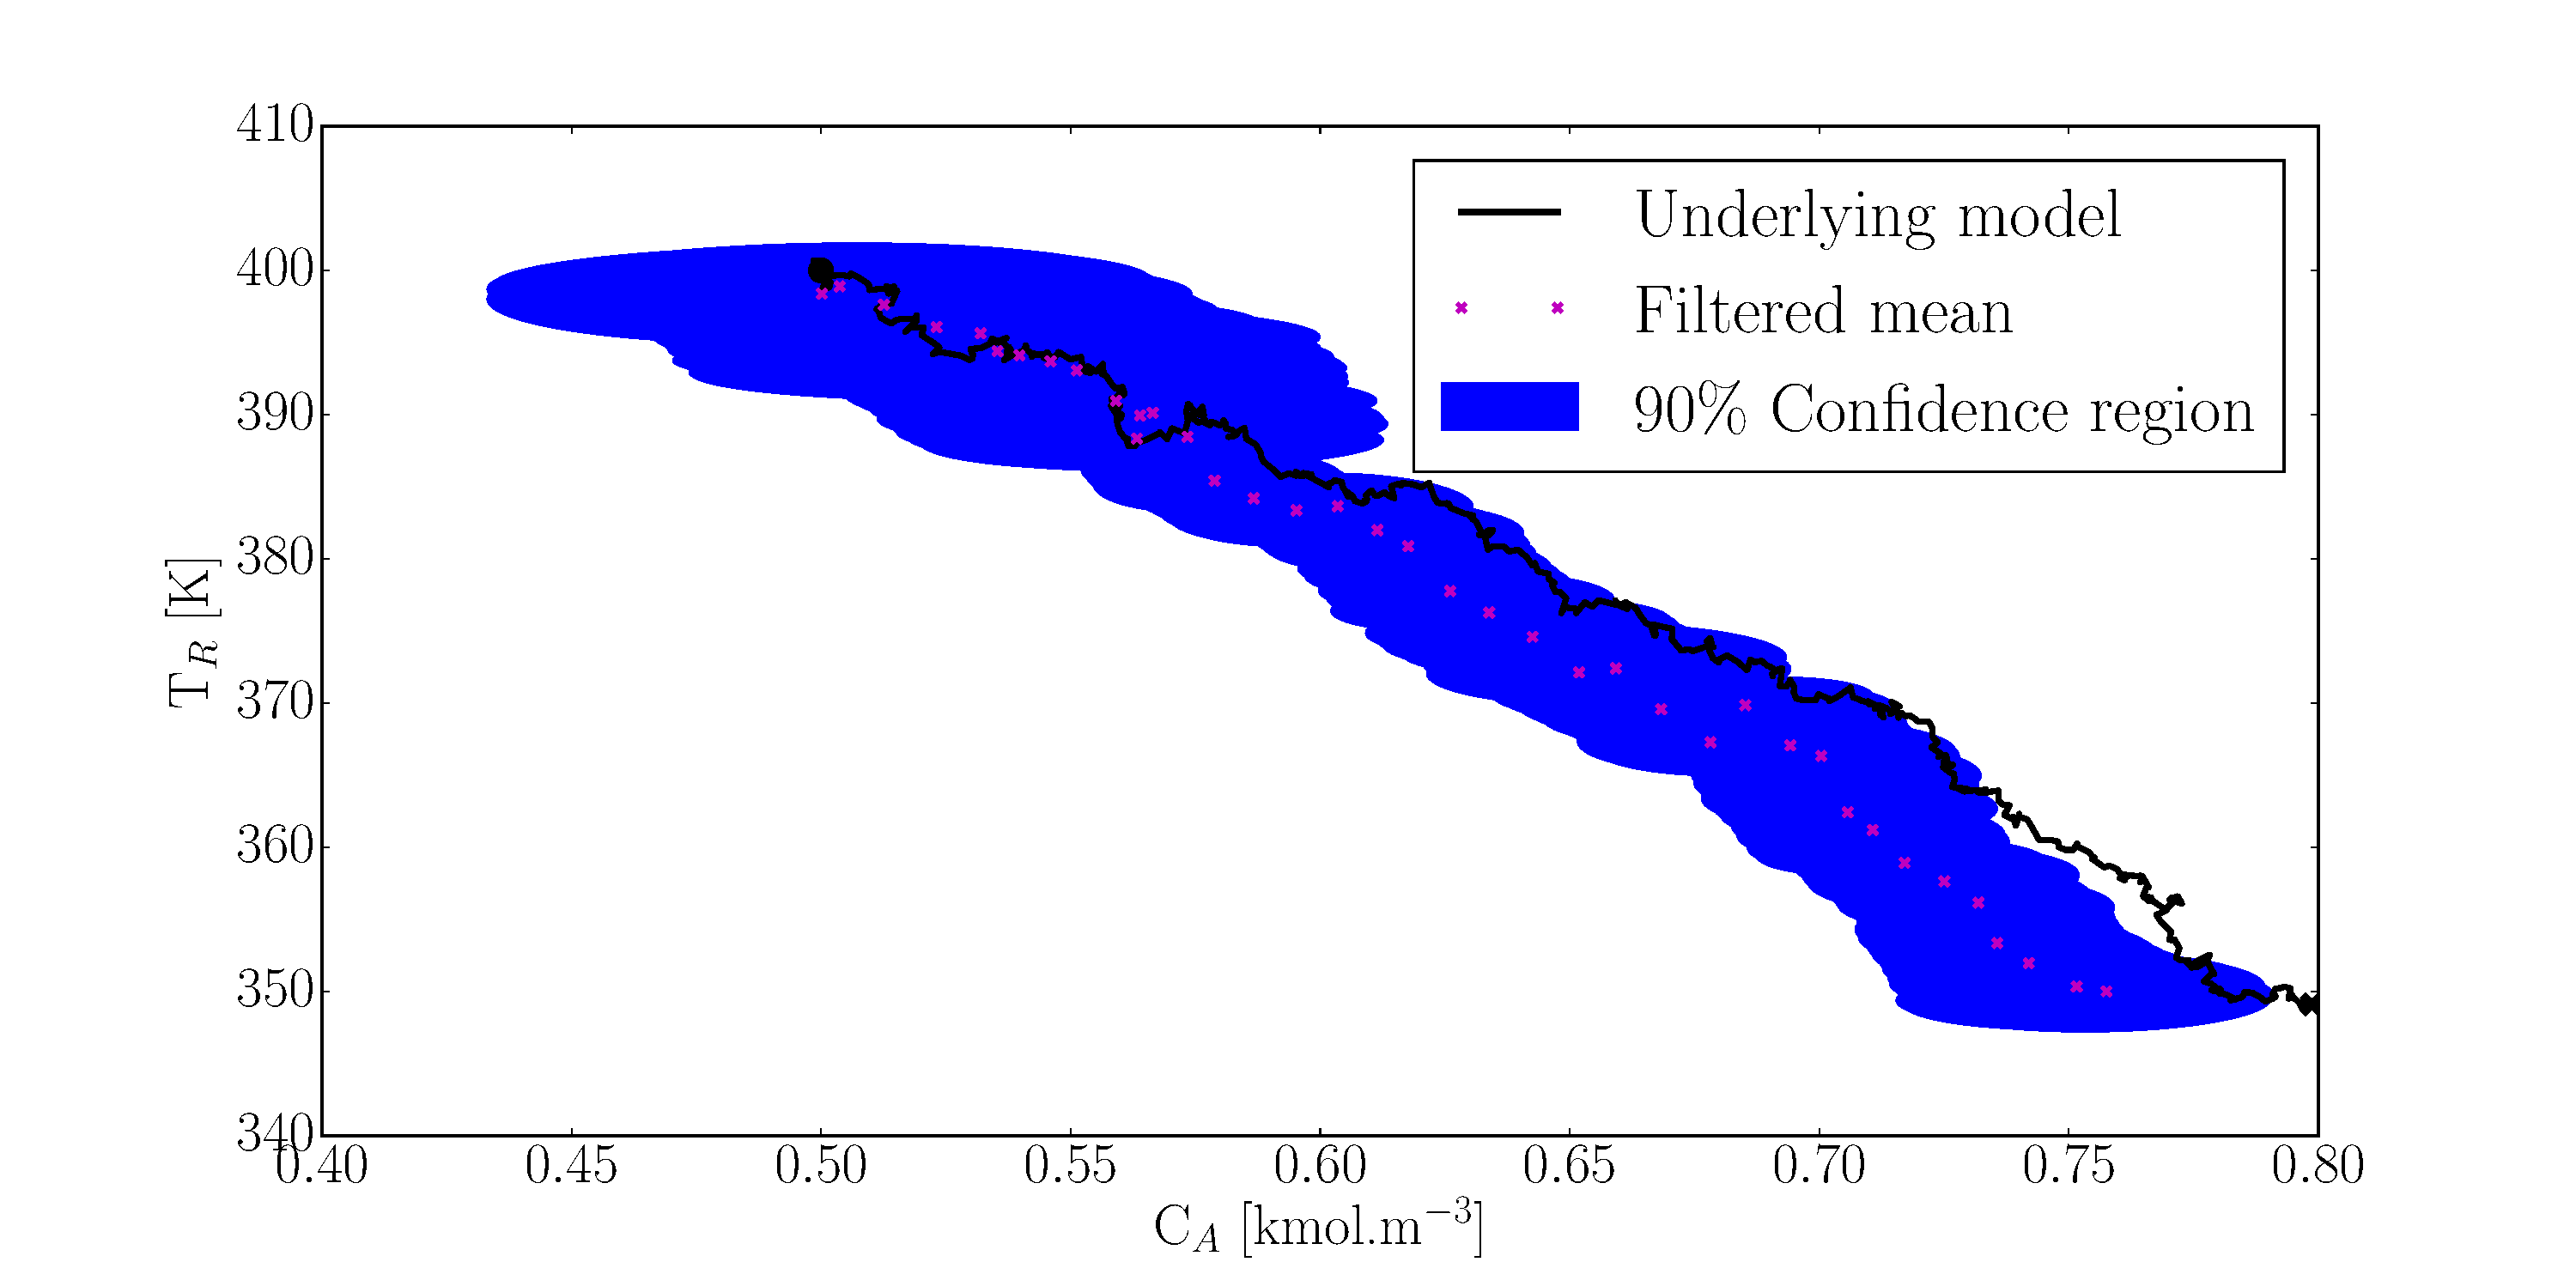
\includegraphics[scale=0.30]{pf_m1_phase.pdf}
\caption{State space evolution of the Particle Filter on the nonlinear CSTR model with initial condition $(0.5, 450)$ and measuring only temperature.}
\label{fig_pf_m1_phase}
\end{figure}
Unfortunately, as Figures \ref{fig_pf_m1_time_bad} and \ref{fig_pf_m1_phase_bad} show, Particle Filters are not a magic bullet for state estimation. In this case we see that the filter tracks the temperature well, as we expect because it is measured, but very poorly estimates the concentration state.
\begin{figure}[H] 
\centering
\includegraphics[scale=0.30]{pf_m1_time_bad.pdf}
\caption{Time series state estimates using the Particle Filter on the nonlinear CSTR model with initial condition $(0.5, 400)$ and measuring only temperature.}
\label{fig_pf_m1_time_bad}
\end{figure}
\begin{figure}[H] 
\centering
\includegraphics[scale=0.30]{pf_m1_phase_bad.pdf}
\caption{State space evolution of the Particle Filter on the nonlinear CSTR model with initial condition $(0.5, 400)$ and measuring only temperature.}
\label{fig_pf_m1_phase_bad}
\end{figure}
The problem we have is that the particles which inaccurately estimate the concentration are not replaced (resampled) because they do not necessarily estimate the temperature poorly. This causes the filter to erroneously believe that all the particles which estimate the temperature correctly are part of the posterior state estimate (should have high weight). This manifests itself in wildly inaccurate state estimates. Since we do not measure the concentration this problem is inherent to the current set up. Therefore we again see that it is better to measure a state (or some effect thereof) than not! 

Finally we compare the Particle Filter to the Kalman filter, using both temperature and concentration measurements. In Figure \ref{fig_pf_kf_time} we see that both the Particle Filter and the Kalman Filter are able to accurately estimate the posterior state distribution. Note that we have used 500 particles to meaningfully compare the distribution estimates.
\begin{figure}[H] 
\centering
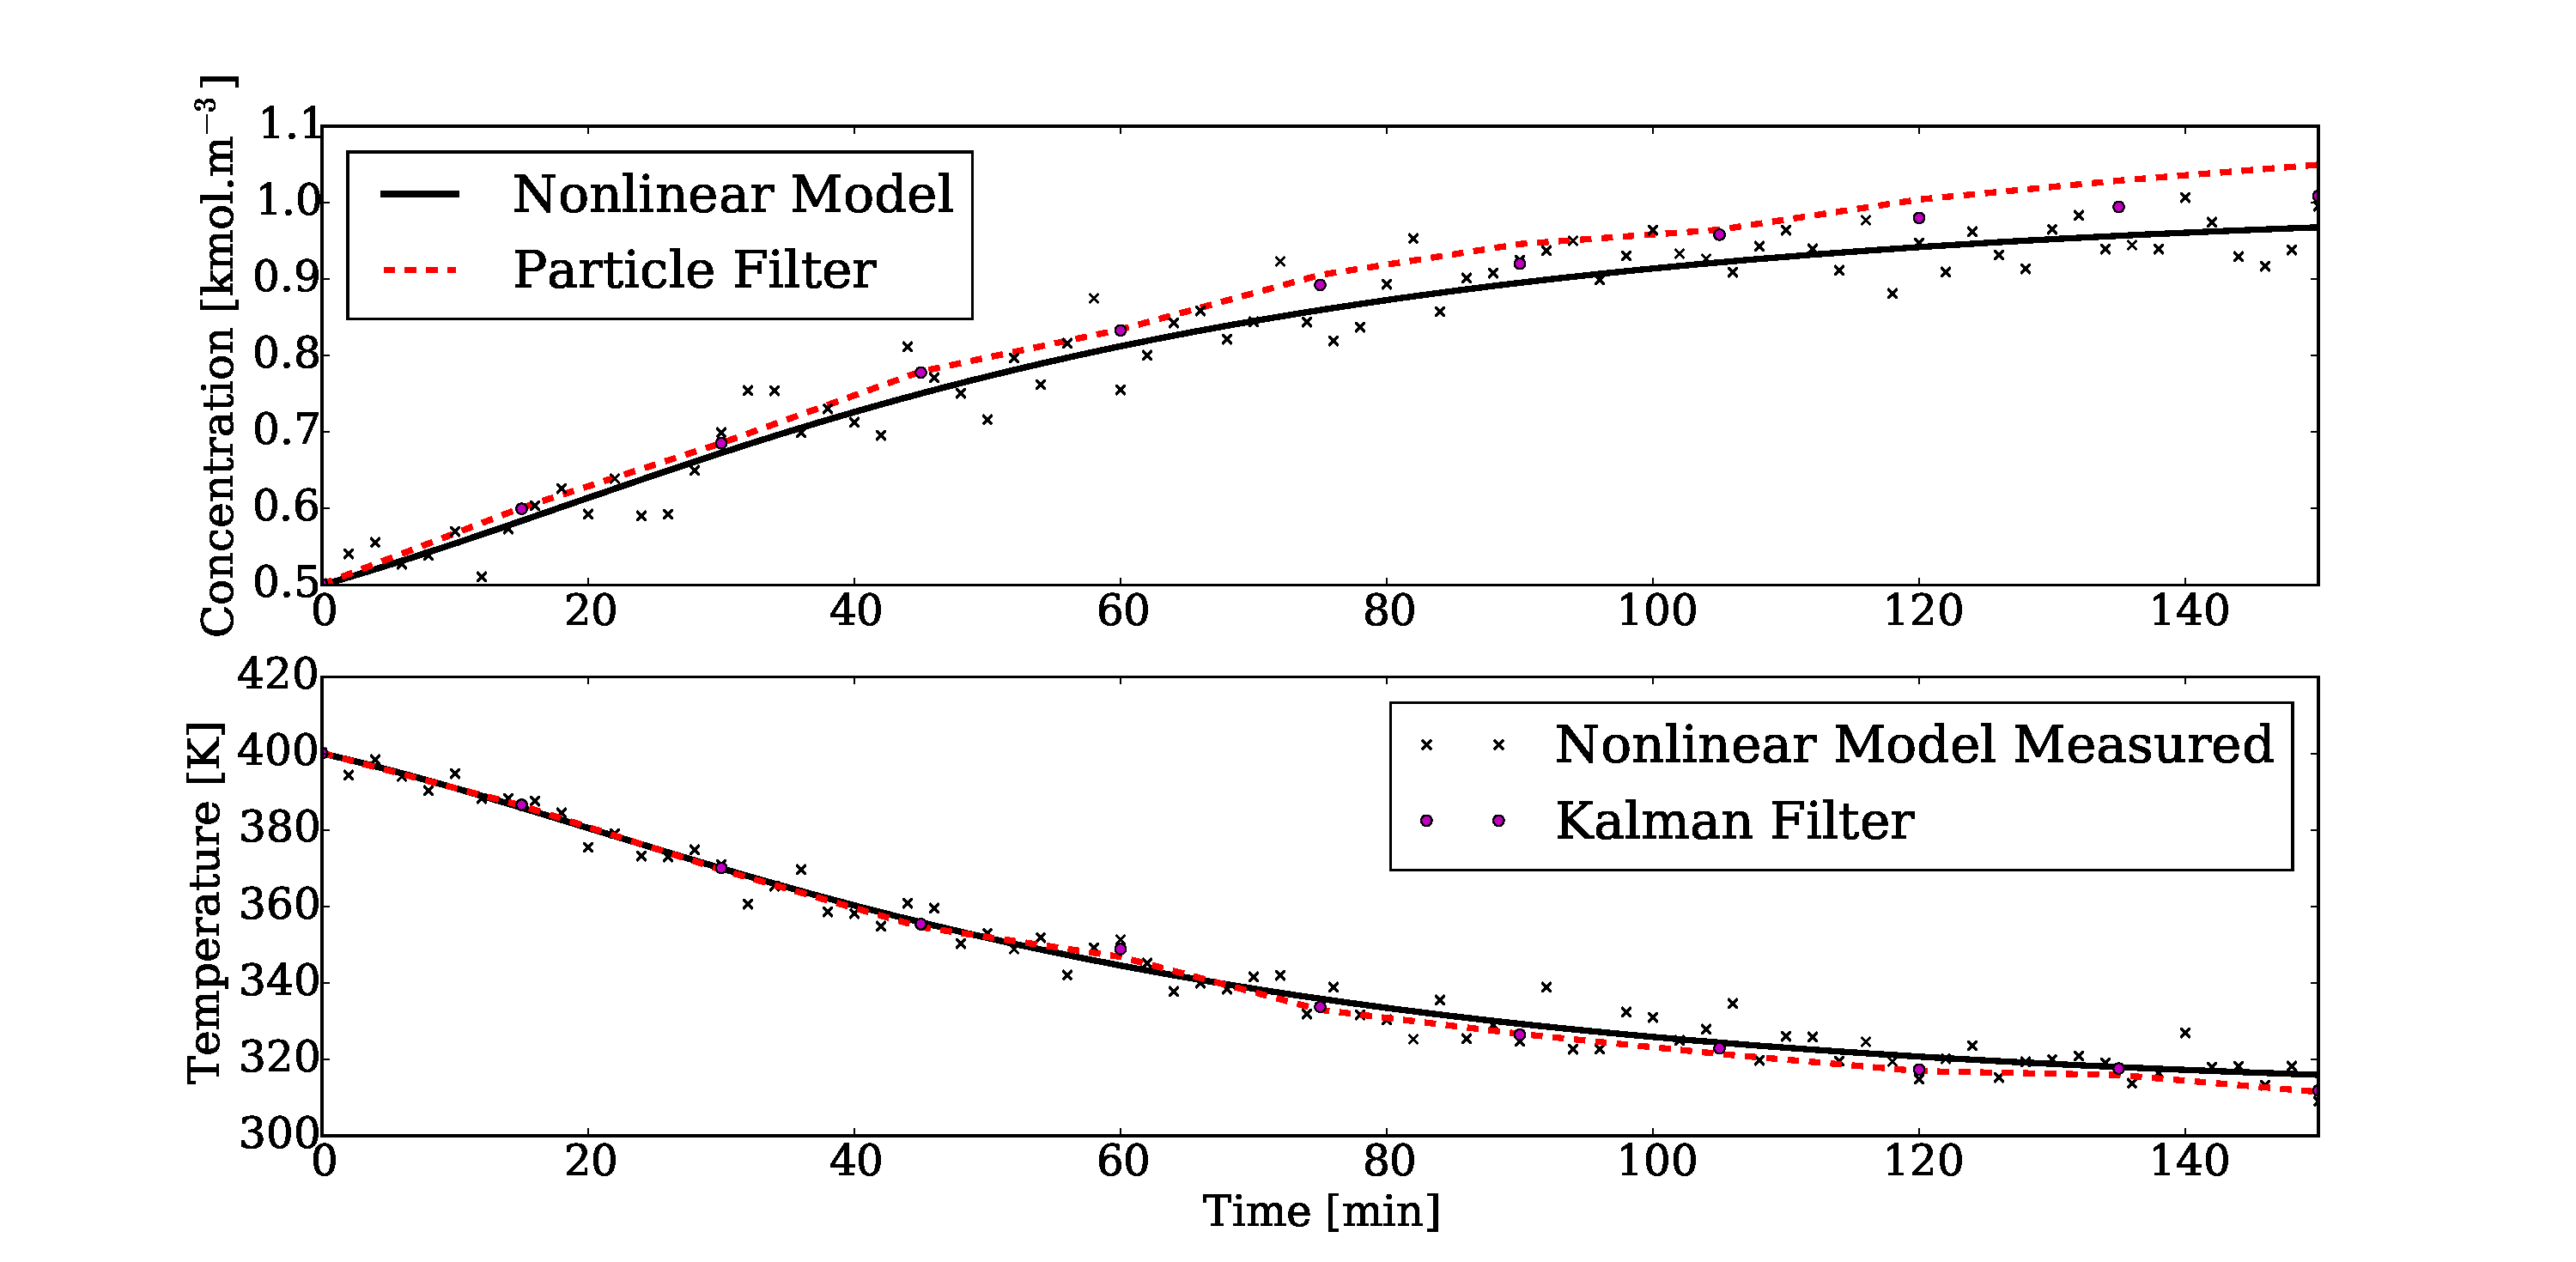
\includegraphics[scale=0.30]{pf_kf_time.pdf}
\caption{Time series state estimates using the Particle Filter and the Kalman Filter on the linear CSTR model (around the unstable operating point) with initial condition $(0.5, 400)$ and measuring only temperature.}
\label{fig_pf_kf_time}
\end{figure}
In Figure \ref{fig_pf_kf_phase} we see empirical proof of the assertion that the Kalman Filter is the optimum state estimator for conditionally linear Gaussian systems \cite{shalom}: the $1\sigma$ ellipses for the Kalman Filter are much smaller than the corresponding ellipses for the Particle Filter. 
\begin{figure}[H] 
\centering
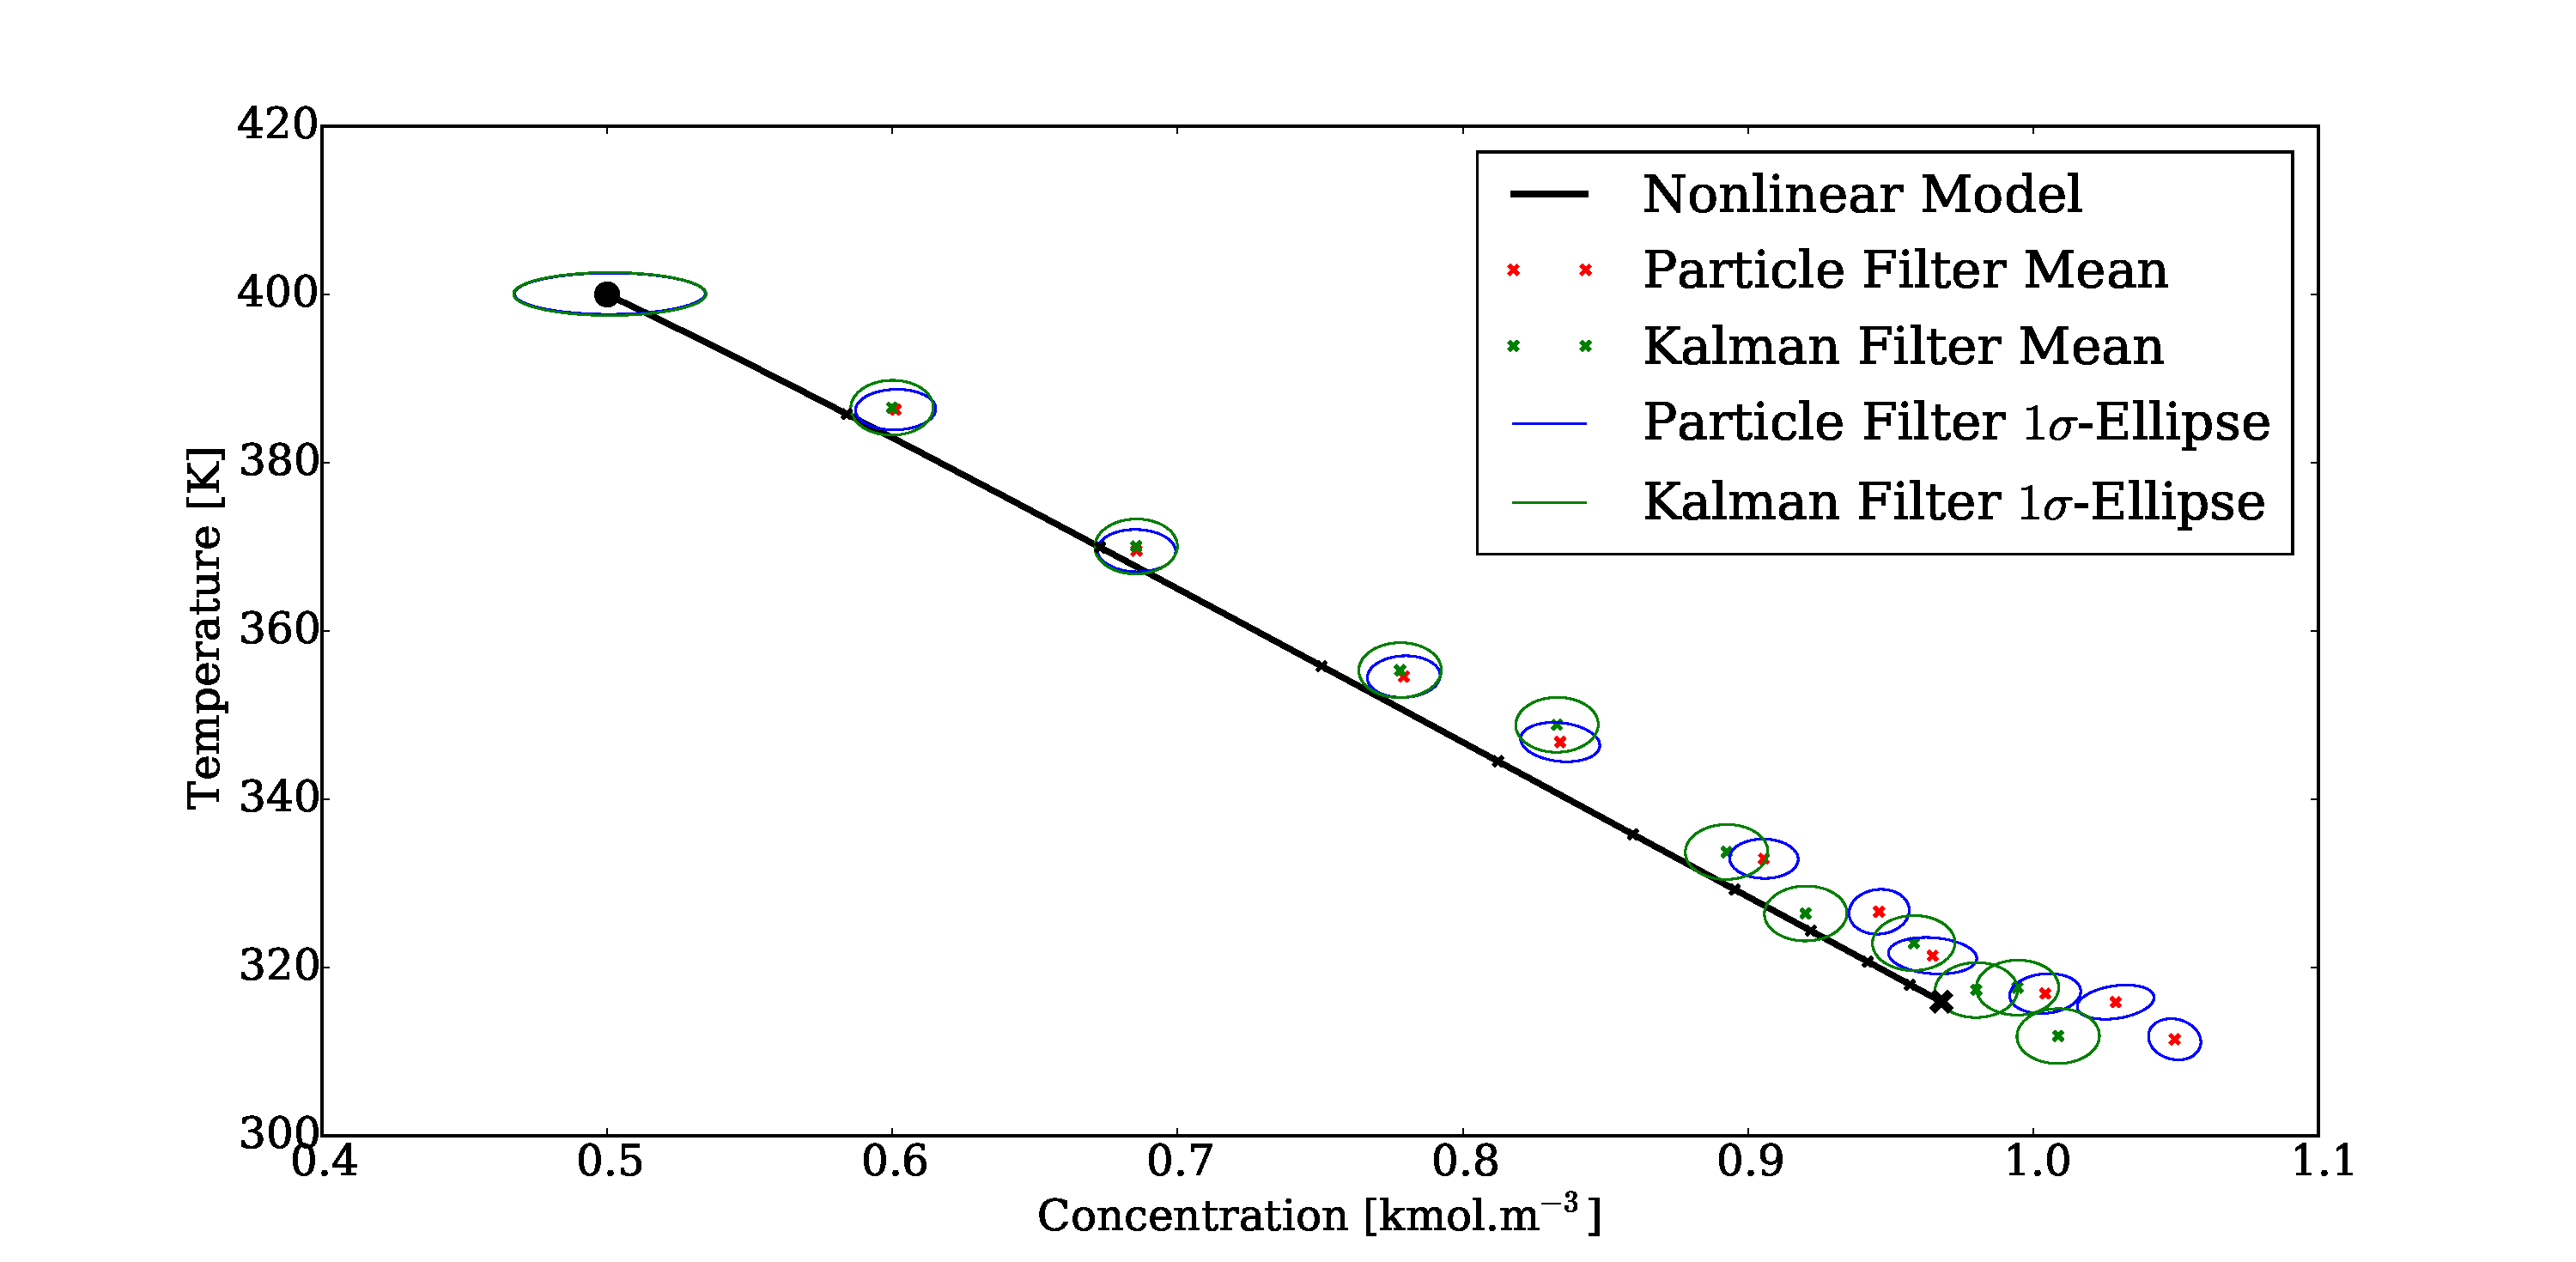
\includegraphics[scale=0.30]{pf_kf_phase.pdf}
\caption{State space evolution of the Particle Filter and the Kalman Filter on the linear CSTR model (around the unstable operating point) with initial condition $(0.5, 400)$ and measuring only temperature.}
\label{fig_pf_kf_phase}
\end{figure}

\bibliographystyle{plain}
\bibliography{research}

\end{document}